\documentclass[11pt]{article}
\usepackage[margin=1in]{geometry}
\usepackage[T1]{fontenc}
\usepackage[utf8]{inputenc}
\usepackage{lmodern,microtype}
\usepackage{amsmath,amssymb,amsthm,mathtools}
\usepackage{graphicx,booktabs,array,enumitem,setspace,placeins}
\usepackage{algorithm}
\usepackage{algpseudocode}
\usepackage{needspace}
\usepackage[authoryear,round]{natbib}
\usepackage{xr-hyper}
\usepackage[colorlinks=true,allcolors=blue]{hyperref}
\usepackage{bookmark}
\allowdisplaybreaks
\setstretch{1.18}
\setlength{\parskip}{0pt}
\setlength{\emergencystretch}{2em}
\setlist{itemsep=2pt,topsep=4pt}
\newtheorem{theorem}{Theorem}[section]
\newtheorem{lemma}[theorem]{Lemma}
\newtheorem{proposition}[theorem]{Proposition}
\newtheorem{corollary}[theorem]{Corollary}
\newtheorem{definition}[theorem]{Definition}
\newtheorem{example}[theorem]{Example}
\theoremstyle{remark}
\newtheorem{remark}[theorem]{Remark}
\newcommand{\E}{\mathbb E}
\newcommand{\Prob}{\mathbb P}
\newcommand{\ind}{\mathbf 1}
\newcommand{\kl}{\operatorname{kl}}
\newcommand{\pos}[1]{\left[#1\right]_+}
\newcommand{\suppproof}{Complete proofs appear in the supplementary material.}

\externaldocument[][nocite]{build/supplement}[supplement.pdf]
% Set \anonymoustrue for an author-free review copy if required by the portal.
\newif\ifanonymous
\anonymousfalse
\title{The Cost of Reliable Near-Optimal Set Maintenance\\with Arriving Arms}
\ifanonymous
\author{}
\else
\author{Deqi Zheng\thanks{The first two authors contributed equally.} \quad
 Xiaoyang Xu\footnotemark[1] \\ Qiuzhen College, Tsinghua University
 \and Yuhong Yang\thanks{Corresponding author: yyangsc@mail.tsinghua.edu.cn.}\\
 Yau Mathematical Sciences Center, Tsinghua University}
\fi
\date{October 15, 2026}
\ifanonymous
\hypersetup{pdftitle={The Cost of Reliable Near-Optimal Set Maintenance with Arriving Arms},pdfauthor={}}
\else
\hypersetup{pdftitle={The Cost of Reliable Near-Optimal Set Maintenance with Arriving Arms},pdfauthor={Deqi Zheng, Xiaoyang Xu, Yuhong Yang}}
\fi
\begin{document}
\maketitle

\begin{abstract}
We study reliable maintenance of all relatively near-optimal arms while
collecting rewards when new arms arrive exogenously and remain available.
Reward laws are stationary, but arrivals change the membership boundary.
Reporting progress is measured by cumulative unresolved arm time outside
a prescribed boundary band, with simultaneous correctness of all labels.
One uncertain arrival can obstruct many earlier certifications. A
common-reference lower bound quantifies this effect, and matching
worst-schedule area bounds yield an arrival-growth boundary for joint
sublinear performance. On specified repeated-update families, temporary
membership tasks impose rapid-maintenance regret costs, while separate
constructions attain deferred and intermediate service levels. We develop
Flexible Certificate-Cost Planning (F-CCP) as a tunable implementation. It
combines sequential evidence and local certificate planning with a chosen
reward kernel and separate observable budgets for reward and
certification. Its guarantees include label reliability, unconditional
expected-regret protection, and service-rate area bounds that retain
budget rejections. Fixed-checkpoint and activation-budgeted constructions
remain distinct analytical witnesses. Frozen paired experiments show
lower mean costs in many finite-budget comparisons, together with
exceptions, heavier regret tails, and nonzero reporting failures. These
results do not characterize a general regret--maintenance frontier.
\end{abstract}
\noindent\textit{Keywords:} sequential experimentation; arriving arms;
near-optimal set maintenance; dynamic regret; confidence sequences.

\section{Introduction}
\label{sec:introduction}

Sequential experiments often acquire new candidates while earlier ones remain
available. An allocation rule must learn which candidates yield high rewards.
An experimenter may also need to know which of all available candidates are
within a specified tolerance of the current best. These objectives need not
favor the same observations. A candidate can be sufficiently inferior to
receive little reward-driven exploration and still be difficult to classify
relative to the near-optimality boundary.

We study these objectives together under permanent exogenous arrivals and
stationary reward laws. If $r^*(t)$ is the largest mean among the arms
available at time $t$, an arm is relatively near-optimal when its mean is at
least $r^*(t)-\varepsilon$. Reports certify membership, certify exclusion, or
leave the arm unresolved. We require one simultaneous correctness event for
all labels at all times. To rule out indefinite abstention, we charge the
cumulative unresolved time of arms whose means lie more than $\eta$ from
the membership boundary. The question is how much regret is necessary, and
how much is attainable, under this reporting requirement.

New arrivals affect the task in two ways. An uncertain new candidate may be
better than the incumbent by enough to invalidate many existing positive
reports. Evidence about that one candidate is then relevant to many
reports at once. A later improvement can also make an earlier difficult
membership question unnecessary: a candidate close to the old boundary may
be far below the new one. Its existing upper confidence bound can be
combined with a new reference's lower bound to certify exclusion. Neither
effect requires the reward law of an old arm to change.

Our observation model and regret comparator have established precedents.
Permanent arrivals form a monotone special case of sleeping-bandit
availability \citep{kleinberg2010}; ballooning bandits already compare reward
with the best arm currently available \citep{ghalme2021}. Exogenous arrivals
differ from drawing arms on demand from a reservoir
\citep{10.1214/aos/1069362389} and from the disappearing actions of mortal
bandits \citep{NIPS2008_788d9869}. Benchmark improvements here arise from new
arms, whereas nonstationary bandits allow the reward distributions of
existing arms to change \citep{Besbes2014,Auer2019ADSWITCH}. Sequential
allocation and adaptive experimentation have a long statistical history
\citep{Robbins1952,LAI19854,Lai1987}; the expanding set of actions retains
that allocation problem and adds an evolving inferential target.

For a fixed arm set, identifying every relatively near-optimal arm is the
ALL-$\varepsilon$ problem \citep{mason2020}. Joint reward and identification
objectives also have established precedents
\citep{degenne2019,yang2026,cho2025}. Our task requires continuing reports
under arrivals, with all-time label reliability and an explicit cumulative
cost for unresolved arm time. The distinction concerns the reporting
protocol and its cost, rather than a new arriving-arm model. The simultaneous
recovery scales used in our lower bounds build on existing information
inequalities and multiple-recovery arguments
\citep{kaufmann2016,malloy2014,jamieson2018}.

We give three results about maintenance cost. First, a common-reference
lower bound shows how one uncertain arrival can obstruct many other
certifications. Its information queue accumulates cost over time within
one reward environment. Second, we obtain matching worst-schedule orders
for cumulative unresolved area, including finite-horizon truncation, and
derive the polynomial arrival boundary for jointly sublinear area and
expected regret. This worst-case lower bound already occurs in an initial
static batch; the common-reference result describes a separate consequence
of continuing arrivals. Third, on a specified repeated-update family,
rapid resolution of temporary membership tasks has matching inverse-square
regret costs. Allowing a constant-factor larger area budget admits a
logarithmic regret upper bound. A nonvanishing-probability lower bound
holds in one fixed environment under the same cumulative-area requirement.
The deferred endpoint has only an upper bound. A separate activation-budgeted
witness covers an intermediate interval on a more strongly separated family;
the general causal frontier under overlapping arrivals remains open.


Fixed checkpoints make attainable costs explicit, but their quotas can
consume a moderate budget before useful reports appear. F-CCP uses every
observation to update valid reporting evidence and plans one certificate
observation at a time. A predictable priority controls the proposed
service rate. Separate budgets limit the virtual-index cost of reward
choices and of certification, so exploration by the reward kernel does
not exhaust the certification account. The resulting guarantees concern
reliability, regret protection, and conditional service bounds; the
local planning proxy is not a solution of the full statistical
allocation problem. The fixed-checkpoint witnesses are retained for
their original guarantees in the supplement.

The components have precedents. Betting processes provide time-uniform
inference for bounded means \citep{waudbysmith2024betting}; our particular
mixture and its bounded-reward validity are proved explicitly.
Thompson sampling supplies a flexible reward rule \citep{thompson1933}.
MOTS obtains fixed-arm minimax guarantees by modifying sampled scores
\citep{jin2021mots}. Our protection instead constrains the virtual-index
cost of the actual selected action under arrivals, and does not transfer
MOTS's theorem to a cold-temperature Beta rule. Conservative bandits
control performance against a fixed baseline \citep{wu2016conservative};
the two accounts here control index deficits and are not realized
shortfalls from a separately run baseline. The spectral accounting and
MC-MOSS concentration tools are inputs from the companion work
\citep{temporalgeometry2026}, not a new characterization claimed here.

Information about future task expiration also matters. A schedule-specific
comparator can defer a temporary question in a way that one causal policy
facing an unknown schedule cannot reproduce uniformly. We retain that
information distinction and an activation-budgeted intermediate-regime
result alongside the general maintenance bounds. The latter uses its own
window conditions and is not an optimality claim for F-CCP.

Section~\ref{sec:model} fixes the joint task and separates task parameters
from allocation preferences. Section~\ref{sec:method} presents F-CCP and
its guarantees. Sections~\ref{sec:maintenance} and~\ref{sec:tradeoff}
give the general costs, temporary-task bounds, and information limits.
Section~\ref{sec:experiments} evaluates frozen configurations, including
mean improvements, tail costs, failed reports, and the corrected
same-controller comparison.
\section{Model, reliable reports, and maintenance cost}
\label{sec:model}
\label{sec:problem}

\subsection{Observation model and regret}

Let $\mathcal A$ be a possibly infinite set of arms. Arm $i$ arrives at
time $\tau_i$, after which it remains available. At every physical time
$t=1,2,\ldots$,
\[
 \mathcal A_t=\{i:\tau_i\le t\},\qquad
 1\le K_t=|\mathcal A_t|<\infty.
\]
Arbitrary finite batches are allowed, including $K_T>T$ at an evaluation
endpoint. Each arm has an unknown stationary reward law on $[0,1]$ with
mean $r_i$. Its successive potential observations $(Y_{i,n})_{n\ge1}$ are
independent and identically distributed, and the streams of different arms
are independent. Arrivals are exogenous and independent of both these
streams and policy randomization. Unless stated otherwise, each result
is for a fixed deterministic arrival schedule.

At time $t$, the policy first receives all current arrivals, then selects
one arm $I_t\in\mathcal A_t$, observes one reward $X_{t,I_t}$, and finally
issues its report. It uses the observed history
\[
 H_{t-1}=(\mathcal A_s,I_s,X_{s,I_s})_{s=1}^{t-1}
\]
and independent randomization. Means, future arrivals, and true membership
labels are unavailable to the policy. With
$N_i(t)=\sum_{s\le t}\ind\{I_s=i\}$, the physical observation is
$X_{t,I_t}=Y_{I_t,N_{I_t}(t-1)+1}$. Write
\[
 \hat r_i(n)=\frac1n\sum_{s=1}^nY_{i,s},\qquad
 r^*(t)=\max_{i\in\mathcal A_t}r_i,\qquad
 \Delta_i(t)=r^*(t)-r_i \quad(i\in\mathcal A_t).
\]
At a deterministic endpoint $T$, cumulative dynamic regret is
\[
 R_T(\pi)=\sum_{t=1}^{T}\Delta_{I_t}(t).
\]
This is a sum of mean gaps, random through the policy's arm selections;
$\E R_T$ is its expectation. The quantity does not compare realized
reward sequences. Physical time always counts actual observations.

\subsection{Reliable reports and cumulative unresolved time}
\label{sec:reporting_task}

For $0<\varepsilon<1$, the target set is
\[
 \mathcal G_t^\varepsilon=\{i\in\mathcal A_t:\Delta_i(t)\le\varepsilon\}.
\]
After the current observation, a report partitions all of $\mathcal A_t$
into $\mathcal P_t,\mathcal N_t,\mathcal V_t$: certified members, certified
nonmembers, and unresolved arms. Define
\[
 E_{\rm lab}=\{\text{for all }t:\ \mathcal P_t\subseteq\mathcal G_t^\varepsilon
                  \subseteq\mathcal A_t\setminus\mathcal N_t\}.
\]
A policy is $\delta$-reliable if $\Prob(E_{\rm lab})\ge1-\delta$ in every
allowed reward environment. A positive report may be withdrawn after a new
arrival. On the correctness event, a negative report remains valid because
$r^*(t)$ is nondecreasing and the arm's mean is stationary.

Reliability permits all arms to remain unresolved. For a boundary width
$0<\eta<1$, define
\begin{equation}
 \begin{split}
 d_i^\varepsilon(t)&=|\Delta_i(t)-\varepsilon|,\\
 U_t(\eta)&=\sum_{i\in\mathcal A_t}
   \ind\{i\in\mathcal V_t,d_i^\varepsilon(t)>\eta\},\qquad
 \mathcal U_T(\eta)=\sum_{t=1}^{T}U_t(\eta).
 \end{split}
 \label{eq:area}
\end{equation}
The count includes newly arrived arms with no observations and old arms
that become unresolved again. Every such arm--time pair is charged; the
loss is not limited to the time before a first decision. Within the
boundary band, unresolved time is exempt, but any label issued there must
still be correct. The true distance $d_i^\varepsilon(t)$ is used only by
the evaluator and in the analysis.

Task parameters are fixed within a comparison. Allocation preferences
change the strategy, rather than the reporting target. The parameters
used below have the following roles.
\begin{center}
\small
\begin{tabular}{lp{.67\textwidth}}
\toprule
Parameter & Role\\
\midrule
$\varepsilon,\eta\in(0,1)$ & Membership tolerance and exempt boundary width\\
$\delta\in(0,1/2)$ & Simultaneous reporting error budget\\
$\lambda_t\in[0,1]$ & Predictable preference for certification\\
$p_0\in(0,1),\ k_0>0,\ \nu>0$ & Service floor, backlog scale, and planning price floor\\
$\mathsf B,\ \theta>0$ & Reward-score kernel and its temperature\\
$\beta_R,\beta_C\in[0,\infty]$ & Fixed reward and certification guard coefficients\\
$\rho$ & Auxiliary checkpoint precision; F-CCP uses $\eta/4$\\
\bottomrule
\end{tabular}
\end{center}
The fixed-checkpoint witnesses may prescribe other precisions before
observations. Preference switching does not change
$\varepsilon,\eta,\delta$, create observations, or reset accumulated
evidence or budget accounts.


The main requirement at a fixed $T$ is
\begin{equation}
 \E_\vartheta R_T\le r,\qquad
 \Prob_\vartheta\{E_{\rm lab},\mathcal U_T(\eta)\le a\}\ge1-\delta.
 \label{eq:joint_protocol}
\end{equation}
It combines an expected regret bound with a joint high-probability
label--area guarantee. In particular, $\mathcal U_T=o(T)$ requires the
time-average number of unresolved separated arms to vanish, rather than
only a small unresolved fraction of all arms. The area guarantee is for
each deterministic endpoint; it need not hold for every endpoint on one
common area event.

For a performance family $\Theta$, let $\mathfrak R_\Theta(a)$ be the
infimum of $\sup_{\vartheta\in\Theta}\E_\vartheta R_T$ over policies reliable on
the full bounded model and satisfying the probability condition in
\eqref{eq:joint_protocol} for every $\vartheta\in\Theta$. The value is
$+\infty$ if the feasible class is empty. Full-model label reliability
and a family-specific area guarantee are distinct requirements. The
lower bounds remain valid when reliability is required only on the
lower-bound subfamily.

\subsection{How arrivals change the reporting problem}

For a fixed old arm, $\Delta_i(t)$ is nondecreasing, so its true membership
can change only from member to nonmember. Its boundary distance
$|\Delta_i(t)-\varepsilon|$ need not be monotone. A new candidate can first
create uncertainty about the current best mean, obstructing positive
certification of many old arms even when those arms remain truly
near-optimal. A sufficiently good new reference can later move the
boundary past earlier candidates, making their fine classification
unnecessary. Sections~\ref{sec:maintenance} and~\ref{sec:tradeoff} quantify
these two effects under the same reporting protocol.


Arms with close means need not be close to the relative boundary
$r^*(t)-\varepsilon$. Conversely, a candidate near that boundary can
require fine evidence even when its reward gap is appreciable. The
algorithm's observable work set is therefore defined from confidence
intervals, not from the evaluator's true gaps or unresolved area.
\section{Flexible certificate-cost planning}\label{sec:fccp}\label{sec:method}
The reporting task need not receive a fixed fraction of every sampling
budget. Evidence obtained while collecting rewards can already certify
some arms, and a small amount of additional work can complete other
reports. Flexible Certificate-Cost Planning (F-CCP) uses one set of lifetime
statistics for both purposes. Its service preference controls how often
certification is attempted; two separate budgets protect the reward
allocation and reserve capacity for certification. The resulting guarantees
concern reliable labels, regret order, and service completion. They do not
identify the optimal allocation for every joint regret--area constraint.

\subsection{Evidence and current reporting work}\label{sec:fccp-evidence}
Order arms by arrival, with a fixed order within each batch. Write
$n_i=N_i(t-1)$ and $\Sigma_i$ for the actual count and reward sum available
before the action at time $t$. Initially $n_i=\Sigma_i=0$ and
$[\ell_i,u_i]=[0,1]$. For $\alpha_i=\delta/\{2i(i+1)\}$, invert the
beta-mixture process
\begin{equation}\label{eq:fccp-mixture}
 \mathsf M_{i,n}(m)=
 \frac{\operatorname B(\Sigma_{i,n}+1/2,n-\Sigma_{i,n}+1/2)}
 {\operatorname B(1/2,1/2)m^{\Sigma_{i,n}}(1-m)^{n-\Sigma_{i,n}}},
 \qquad m\in[0,1],
\end{equation}
where $\operatorname B$ is the beta function, distinguished from the
optimal mean $r^*(t)$. The interval is the intersection of
$\{m:\mathsf M_{i,n}(m)\le1/\alpha_i\}$ over all observed positive
prefixes. At the actual count
\begin{equation}\label{eq:fccp-quota}
 \rho=\eta/4,\qquad
 q_i=\left\lceil\frac{2}{\rho^2}
             \log\frac{4i(i+1)}{\delta}\right\rceil,
\end{equation}
intersect it also with
$[\hat r_i(q_i)-\rho/2,\hat r_i(q_i)+\rho/2]\cap[0,1]$.
Continue the mixture updates after this checkpoint. The construction is
valid for bounded rewards, including nonbinary rewards; its supermartingale
argument is given in Supplement~\ref{app:fccp-evidence}. Sequential betting
and mixture confidence sequences are established tools
\citep{waudbysmith2024betting}.

For a nonempty confidence rectangle define
\begin{equation}\label{eq:fccp-gap}
 g_i^-=\max\{0,\max_{j\ne i}\ell_j-u_i\},\qquad
 g_i^+=\max\{0,\max_{j\ne i}u_j-\ell_i\}.
\end{equation}
Both bounds are zero when there is only one arm. They are the exact
minimum and maximum of the gap over this rectangle, including its
self-exclusion constraint. After observing a reward, report
\begin{equation}\label{eq:fccp-report}
 \mathcal P_t=\{i:g_i^+\le\varepsilon\},\quad
 \mathcal N_t=\{i:g_i^->\varepsilon\},\quad
 \mathcal V_t=\mathcal A_t\setminus(\mathcal P_t\cup\mathcal N_t).
\end{equation}
A negative report does not remove an arm from future reward allocation.
Among unresolved arms let
\begin{equation}\label{eq:fccp-work}
 Z_t=\{i\in\mathcal V_t:[g_i^-,g_i^+]
                 \subseteq[\varepsilon-\eta,\varepsilon+\eta]\},
 \qquad W_t=\mathcal V_t\setminus Z_t.
\end{equation}
These formulas are also evaluated before the action, after the current
arrivals, when choosing that round's service. An arm in $Z_t$ remains
reported as unresolved; the rectangle already shows that it incurs no
$\eta$-unresolved cost. Recompute the sets after every arrival and
observation. An empty interval sets a persistent failure flag: all
subsequent reports are unresolved and designated service stops. Reward
allocation, its guard, and the actual statistics continue.

\subsection{A local certificate plan}\label{sec:fccp-plan}
The plan assigns observations a positive price and asks which current
pairwise certificate is cheapest to pursue. Its centers and radii are
\begin{equation}\label{eq:fccp-planning}
 m_i=\Pi_{[\ell_i,u_i]}\frac{\Sigma_i+1/2}{n_i+1},\quad
 v_i^{\mathrm{plan}}=\max(m_i-\ell_i,u_i-m_i),\quad
 \bar n_i=\max(1,n_i).
\end{equation}
Here $\bar n_i$ is a planning convention; no fictitious observation enters
the confidence interval. For each $i\in W_t$, take as its reference $j$
the arm of largest $m_j$ if $\max_km_k-m_i>\varepsilon$; otherwise take
the largest-upper-bound arm other than $i$. Resolve reference ties by arrival
order. Set
\begin{equation}\label{eq:fccp-price}
 h_i=.95\max\{|m_j-m_i-\varepsilon|,
                   \eta-|m_j-m_i-\varepsilon|\},\quad
 c_k=\nu+(1-\lambda_t)\zeta_t(k),\quad
 a_k=v_k^{\mathrm{plan}}\sqrt{\bar n_k},
\end{equation}
where $\nu>0$ and the observable index gap $\zeta_t$ is defined below.
Solve the two-coordinate proxy problem
\begin{equation}\label{eq:fccp-pair}
 \min_{x_i\ge\bar n_i,\,x_j\ge\bar n_j}
  c_i(x_i-\bar n_i)+c_j(x_j-\bar n_j)
 \quad\text{subject to}\quad
  a_i/\sqrt{x_i}+a_j/\sqrt{x_j}\le h_i.
\end{equation}
The interior solution is explicit; boundary and zero-radius cases appear
in Supplement~\ref{app:fccp-evidence}. Among pairs with an available
endpoint, use the pair of smallest proxy cost. Within that pair, select
the endpoint maximizing $v_k^{\mathrm{plan}}/(\bar n_kc_k)$ among those
with $n_k<q_k$ and $x_k>n_k$ (using the actual count). Execute only one pull,
then replan. If no pair provides an endpoint, select the widest interval
among arms with $n_k<q_k$, with arrival order breaking ties. Call this
subroutine $\operatorname{Plan}_t$, and its proposed arm $j_t$.

The optimization in \eqref{eq:fccp-pair} is exact for its continuous
proxy. It holds the centers fixed and approximates radius reduction by
an inverse square root. Other competitors can remain after one pair is
resolved. Thus its solution is a scheduling rule, not an information
complexity or a proof of optimal statistical allocation.

\subsection{Virtual indices and two budgets}\label{sec:fccp-budgets}
The reward guard uses a virtual, clipped MC-MOSS index. Its arrival clock
and spectral comparison come from the companion study
\citep{temporalgeometry2026}. Initialize $\mathrm{base}=0$. After arrivals,
if $K_t>1$ and either $\mathrm{base}=0$ or $K_t-1\ge2\,\mathrm{base}$,
set $\mathrm{base}=K_t-1$, $\sigma=t$, and
$d_{\mathrm{clock}}=2\,\mathrm{base}$. Retain all observations. With
$s=t-\sigma+1$, define
\begin{equation}\label{eq:fccp-index}
 J_i(t)=\begin{cases}
 1,&n_i=0,\\
 \min\{1,\hat r_i(n_i)+
       \sqrt{[\log\{s/(d_{\mathrm{clock}}n_i)\}]_+/n_i}\},&n_i>0,
 \end{cases}\qquad
 \zeta_t(i)=\max_jJ_j(t)-J_i(t).
\end{equation}
When $K_t=1$, set $J_i=1$ and $\zeta_t(i)=0$ without using an
uninitialized clock. The virtual index never forces an observation by
itself. In particular, $\zeta_t$ is an observable index difference,
not realized regret or a difference between two independent runs.

Choose the first initial arm as a counting anchor. Among all other
arrived arms, let $k_{\ell,t}$ count current ages $t-\tau_i+1$ in group
$0$ (age one), or group $\ell\ge1$ (ages in
$(2^{\ell-1},2^\ell]$). The current spectrum and its running maximum are
\begin{equation}\label{eq:fccp-spectrum}
 \mathcal S_t=\sum_{\ell\ge0}
       \min\{2^\ell,\sqrt{k_{\ell,t}2^\ell}\},\qquad
 \overline{\mathcal S}_t=\max_{u\le t}\mathcal S_u.
\end{equation}
The anchor's identity supplies no information about its mean or
optimality. Computing \eqref{eq:fccp-spectrum} uses only arrived arms'
current ages, with no endpoint or future-arrival input.

Fix $\beta_R,\beta_C\in[0,\infty]$ before the run. Maintain separate
ledgers, initially zero,
\begin{equation}\label{eq:fccp-ledgers}
 C_R(t)=\sum_{u\le t:\,\mathrm{reward}}\zeta_u(I_u),\qquad
 C_C(t)=\sum_{u\le t:\,\mathrm{service}}\zeta_u(I_u).
\end{equation}
Accept a proposed service only if
$C_C(t-1)+\zeta_t(j_t)\le\beta_C\overline{\mathcal S}_t$.
Otherwise use a reward round and record a denial. On any reward round
maximize the selected reward kernel's scores over
\begin{equation}\label{eq:fccp-feasible}
 \mathcal F_R(t)=\{i:C_R(t-1)+\zeta_t(i)
                                  \le\beta_R\overline{\mathcal S}_t\}.
\end{equation}
A largest-$J_i$ arm has zero index gap, so this set is nonempty. An infinite
budget disables the corresponding check, including when the spectrum is
zero; it is implemented as \texttt{None}, rather than as budget zero.
No ledger is reset at a clock change or preference change.

For example, the default reward scores are one draw per arm,
\begin{equation}\label{eq:fccp-score}
 \Xi_i(t)\sim\operatorname{Beta}
       (1+\Sigma_i/\theta,\,1+(n_i-\Sigma_i)/\theta).
\end{equation}
For Bernoulli rewards, $\theta=1$ gives standard Beta$(1,1)$ Thompson
sampling \citep{thompson1933}; $\theta=.5$ is a colder action rule.
For general bounded rewards these fractional-count scores are a
sampling heuristic. The evidence always uses the original counts and
reward sums. On a reward round draw the full score vector once, then
maximize that same vector over \eqref{eq:fccp-feasible}; do not redraw
following rejection. UCB1, Growing-MOSS, MC-MOSS, and KL-UCB can also
supply reward scores.

\subsection{Service preference and executable rule}\label{sec:fccp-modes}
Let $\lambda_t\in[0,1]$ be a predictable service preference. Given a
proposed service $j_t$, write $b_t=|W_t|$ and
$\widehat c_t=\max_i m_i-m_{j_t}$. The adaptive controller uses
\begin{equation}\label{eq:fccp-rate}
 w_t=p_0+(1-p_0)\frac{b_t}{b_t+k_0}
                         \frac{\varepsilon}{\varepsilon+\widehat c_t},
 \qquad
 p_t=\begin{cases}
 0,&b_t=0\text{ or service is disabled},\\
 \displaystyle\frac{\lambda_tw_t}{1-\lambda_t+\lambda_tw_t},&\text{otherwise}.
 \end{cases}
\end{equation}
Fixed-rate control instead uses $p_t=\lambda_t\ind\{b_t>0\}$.
Service is disabled when the failure flag is set or $\lambda_t=0$.
The presets use $p_0=.02$, $k_0=4$, and $\nu=.1$.
Few or costly proposed certificates tend to reduce the service rate;
a large, inexpensive backlog tends to increase it. The controller sees
$W_t$, not the true unresolved area. Neither $\lambda_t$ nor $w_t$ is
an estimated optimal multiplier or a forecast of future arrivals.

Use a phase $\phi_0=0$: add $p_t$ each round, and if the result is at
least one, attempt one service and subtract one. A denial does not
refund this phase. In exact arithmetic the number of attempts through
$T$ is $\lfloor\sum_{t\le T}p_t\rfloor$. For fixed $\lambda>0$,
on busy rounds,
\begin{equation}\label{eq:fccp-pmin}
 p_t\ge p_{\min}(\lambda):=
          \frac{\lambda p_0}{1-\lambda+\lambda p_0}>0.
\end{equation}
There is no positive service lower bound at $\lambda=0$.
Table~\ref{tab:fccp-modes} separates the four presets. Changing only
\texttt{set\_priority(1)} does not disable an existing certification
budget. Preference changes occur between completed physical rounds and
retain the phase, evidence, counts, and both ledgers.

\begin{table}[t]
\centering\small
\caption{F-CCP presets. The default reward kernel is Beta sampling.
An inactive service budget is never checked because service is off.
The guarantees refer to the conditions stated in this section.}
\label{tab:fccp-modes}
\begin{tabular}{lcccc}
\toprule
Preset (data ID)&$\lambda$/control&$\theta$&$\beta_R$&$\beta_C$\\
\midrule
Reward (F-R)&0/off&.5&16&inactive\\
Balanced (F-auto-0.6)&.6/adaptive&.5&16&1\\
Classification (F-area)&1/fixed&.5&16&$\infty$\\
Compatibility (F-R-TS-exact)&0/off&1&$\infty$&inactive\\
\bottomrule
\end{tabular}
\end{table}

\begin{algorithm}[tbp]
\caption{Flexible certificate-cost planning (F-CCP)}\label{alg:flexible-ccp}
\footnotesize
\begin{algorithmic}[1]
\Require Fixed $\varepsilon,\eta,\delta$, budgets $\beta_R,\beta_C$,
reward kernel, temperature, controller parameters; predictable $\lambda_t$.
\State Initialize empty arm statistics, intervals, and quotas;
$\mathrm{base}=0$, $\phi=C_R=C_C=\overline{\mathcal S}=0$; failure $=\mathrm{false}$.
\For{each physical time $t=1,2,\ldots$}
 \State Admit the current batch in arrival order with $n_i=\Sigma_i=0$,
 $[\ell_i,u_i]=[0,1]$, birth $t$, and quota \eqref{eq:fccp-quota}.
 \State Update the arrival clock and calculate $J_i(t),\zeta_t(i)$
 using \eqref{eq:fccp-index} (use the singleton convention).
 \State Update $\overline{\mathcal S}\gets
 \max\{\overline{\mathcal S},\mathcal S_t\}$ using current ages.
 \State Set attempt $=\mathrm{false}$, service $=\mathrm{false}$, $p_t=0$.
 \If{not failed and $\lambda_t>0$}
  \State Recompute the pre-action reports and $W_t$ from current intervals.
  \If{$W_t\ne\varnothing$}
   \State $j_t\gets\operatorname{Plan}_t$ using
   \eqref{eq:fccp-planning}--\eqref{eq:fccp-pair}; calculate $p_t$.
   \State $\phi\gets\phi+p_t$.
   \If{$\phi\ge1$}
    \State $\phi\gets\phi-1$; attempt $=\mathrm{true}$.
   \EndIf
  \EndIf
 \EndIf
 \If{attempt and a legal $j_t$ exists}
  \If{the service guard is off or
  $C_C+\zeta_t(j_t)\le\beta_C\overline{\mathcal S}$}
   \State $I_t\gets j_t$; service $=\mathrm{true}$;
   $C_C\gets C_C+\zeta_t(I_t)$.
  \Else
   \State Record one service denial; retain the decremented phase.
  \EndIf
 \EndIf
 \If{not service}
  \State Generate the reward score vector once from the current actual history.
  \State $I_t\gets$ first maximizer of these scores over $\mathcal F_R(t)$
  (all $\mathcal A_t$ when that guard is off).
  \State $C_R\gets C_R+\zeta_t(I_t)$.
 \EndIf
 \State Pull $I_t$ once; observe $X_{t,I_t}$;
 $n_{I_t}\gets n_{I_t}+1$, $\Sigma_{I_t}\gets\Sigma_{I_t}+X_{t,I_t}$.
 \If{not failed}
  \State Intersect the selected arm's interval with its new mixture interval;
  at $n_{I_t}=q_{I_t}$ also intersect the fixed-prefix interval.
  \State If any interval is empty, set failure $=\mathrm{true}$ permanently.
 \EndIf
 \State Report \eqref{eq:fccp-report}, or
 $(\varnothing,\varnothing,\mathcal A_t)$ if failed.
\EndFor
\end{algorithmic}
\end{algorithm}

Within a planned pair, equal endpoint scores favor the candidate $i$;
other ties use the fixed arrival-order scans. The procedure sees no
means, hidden identities, future arrivals, or endpoint. Stopping at an
arbitrary endpoint leaves the last completed report unchanged. Its
straightforward implementation takes $O(K_t^2)$ work per round when pair
planning or the self-excluding gap bounds are evaluated by nested scans,
and $O(K_t)$ stored arm statistics. Numerical root finding and floating
comparisons are described separately in the supplement.

\FloatBarrier
\subsection{Reliability, reward protection, and service completion}
\begin{proposition}[Reliable reports]\label{prop:fccp-report}
Under the bounded stationary model, every legal predictable choice of
preferences, prices, and service actions in F-CCP satisfies
$\Prob(E_{\mathrm{lab}})\ge1-\delta$. On a common event
$\mathcal E$ of this probability, all confidence intervals cover their
means at all observed counts, all reports are correct, and every arm in
$Z_t$ lies in the boundary band.
\end{proposition}
The evidence argument does not require the proxy plan to predict its
actual sampling cost. The mixture and checkpoint errors each receive
$\delta/2$, and a union bound gives $\mathcal E$.

\begin{proposition}[Compatibility endpoint]\label{prop:fccp-compat}
Fix a legal reward kernel $\mathsf B$. If service is off from the start
($\lambda_t\equiv0$), $\beta_R=\infty$, and the complete kernel state,
initialization, and random-number source agree with those of
$\mathsf B$, the two procedures have identical actions, lifetime counts,
and regret on every potential reward realization and arrival schedule.
\end{proposition}
This is a same-backend pathwise statement. A common seed in different
random-number backends does not provide the required coupling. The
colder, guarded F-R preset is distinct from this endpoint. Switching off
service after using it does not recreate a baseline's independent past.

The regret comparison uses an arbitrary-action inequality,
\begin{equation}\label{eq:fccp-optimism}
 \E R_T\le\min\left\{T,300\mathcal S_T+
                          \E\sum_{t\le T}\zeta_t(I_t)\right\}.
\end{equation}
Supplement~\ref{app:optimism-gap} proves the bridge from the companion
MC-MOSS potential-prefix and arrival-clock bounds to arbitrary actions;
the potential-prefix bounds apply to the actual sequence of selected actions.

\begin{theorem}[Two-budget reward protection]\label{thm:fccp-budget}
Fix finite nonnegative $\beta_R,\beta_C$ and use legal pre-observation
actions. For every deterministic schedule and endpoint,
\begin{equation}\label{eq:fccp-regret-finite}
 \E R_T\le\min\{T,(300+2\beta_R+2\beta_C)\mathcal S_T\}.
\end{equation}
If service is off throughout the run, omit $2\beta_C$ even when its guard is disabled.
If $\beta_R<\infty$ and $\beta_C=\infty$, then, with
$Q_T^{\mathrm{cap}}=\sum_{i\in\mathcal A_T}q_i$,
\begin{equation}\label{eq:fccp-regret-unlimited}
 \E R_T\le\min\{T,(300+2\beta_R)\mathcal S_T+Q_T^{\mathrm{cap}}\}.
\end{equation}
These bounds are unconditional, including reporting failures.
\end{theorem}
The ledgers satisfy their respective running-spectrum budgets, and
$\overline{\mathcal S}_T\le2\mathcal S_T$.
Substitution in \eqref{eq:fccp-optimism} proves the finite-budget bound.
Unlimited certification costs at most $Q_T^{\mathrm{cap}}$ actual
service pulls. Thus F-R has the conservative bound $332\mathcal S_T$,
Balanced has $334\mathcal S_T$, and Classification retains the extra
$Q_T^{\mathrm{cap}}$ term. The companion spectral minimax lower bound
makes the finite-budget regret order sharp, for fixed coefficients;
the spectral characterization itself is an existing input
\citep{temporalgeometry2026}. None of these bounds compares F-CCP's
realized regret with an independently run Thompson sampler.

\begin{theorem}[Area under a positive service rate]\label{thm:fccp-area}
Suppose every pre-action busy round has $p_t\ge p_{\min}>0$.
Let $D_T^{\mathrm{srv}}$ be the number of service attempts rejected by
the certification budget. On $\mathcal E$, simultaneously at every
endpoint,
\begin{equation}\label{eq:fccp-area}
 \mathcal U_T(\eta)\le K_T\min\left\{T,
                  \frac{Q_T^{\mathrm{cap}}+D_T^{\mathrm{srv}}+1}{p_{\min}}
                                      \right\}.
\end{equation}
When $D_T^{\mathrm{srv}}=0$, this is
$O(\min\{K_TT,K_T^2\eta^{-2}\log(K_T/\delta)/p_{\min}\})$.
\end{theorem}
Here busy means that the current $W_t$ is nonempty after arrivals and
before observation. If every current arm has reached its checkpoint,
the gap intervals are narrow enough that $W_t$ is empty. Each successful
service therefore advances a finite remaining checkpoint, and phase
accounting bounds the number of busy rounds. This proves the theorem
without requiring a cost-optimal plan. Classification has $p_{\min}=1$
and no refusals, hence the worst-area order matches the general lower
bound in its common parameter range. Finite-budget Balanced must retain
the denial term; it has no unconditional prescribed-area guarantee.
An arbitrary predictable $\lambda_t$ preserves label reliability, but
completion speed needs the displayed positive lower bound.

\begin{corollary}[Finite-arm completion]\label{cor:fccp-finite}
Suppose $\beta_C>0$ is fixed, busy rounds have a uniform positive service
rate, and arrivals eventually stop with finitely many arms. On
$\mathcal E$, every arm outside the boundary band eventually receives
a definite label. This conclusion holds regardless of continuing
reward-kernel exploration and its separate ledger consumption.
\end{corollary}
A conservative finite-prefix bound, the compatibility proof, and a
one-round obstruction to exact all-environment dominance appear in
Supplement~\ref{app:fccp-guarantees}. Completion on a fixed-confidence
event concerns the boundary band; it is not unconditional almost-sure
consistency for the exact oracle set.
\section{Fundamental costs of continual maintenance}
\label{sec:maintenance}

\subsection{One uncertain arrival can obstruct many reports}

The first lower bound retains one reward environment throughout the time axis.
It therefore measures a cumulative burden without adding the worst cases of
incompatible experiments. Fix
$0<\varepsilon\le1/16$, $0<\delta\le1/16$, and $0<\eta<\varepsilon/2$.
An initial reference has Bernoulli mean $1/4+\varepsilon/2$. Candidates arrive
on any prescribed schedule. In environment zero each has mean $p=1/4$;
environment $j$ changes only candidate $j$ to mean $p+2\varepsilon$.
All candidates are good in environment zero, with boundary distance
$\varepsilon/2$. After candidate $j$ arrives in environment $j$, every other
candidate is bad.

Let $M_t$ count arrived candidates and $a_t=M_t-M_{t-1}$. Define
\begin{align}
 q_-&=\left\lfloor\frac{\kl(1/4,\delta)}
                              {\kl(1/4,1/4+2\varepsilon)}\right\rfloor,
 &Q_t&=(Q_{t-1}+q_-a_t-1)_+,\quad Q_0=0,\notag\\
 \mathcal B_T&=\sum_{t\le T}(M_t-1)_+\ind\{Q_t>0\}.
 \label{eq:broadcast_queue}
\end{align}
This analytical queue is an information-capacity certificate: arrivals add
$q_-$ units per candidate, while only one observation is possible per round.
It is distinct from F-CCP's phased service rule and from the
fixed-checkpoint witness's FIFO queue. It imposes no pathwise sampling
quota on every candidate. In the stated
range $q_-\ge2$.

\begin{theorem}[Broadcast uncertainty]
\label{thm:broadcast}
For every policy reliable on environment zero and all its one-candidate
alternatives,
\[
 \E_0\mathcal U_T(\eta)\ge(3/4-\delta)\mathcal B_T.
\]
If $\mathcal B_T>0$, then
\[
 \Prob_0\{\mathcal U_T(\eta)\ge\mathcal B_T/4\}\ge1/4.
\]
These conclusions still hold when the policy knows the full arrival schedule,
the horizon, and the reference distribution.
\end{theorem}

At a busy time, some deterministic candidate label has expected sample count
below $q_-$. Changing that candidate alone has too little history KL to permit
positive certification of another candidate with probability at least $1/4$.
Reliability also bounds incorrect negative reports. The remaining probability
must be unresolved. The same reference environment supports this argument at
every time; the difficult label is selected from expected counts rather than
from a favorable realized history. The supplementary proof includes the
bounded-variable step needed for the probability statement.

If $m$ candidates have arrived by time $s$, the queue obeys the deterministic
inequality
\begin{equation}
 \sum_{t\le s+qm-1}(M_t-1)_+\ind\{Q_t(q)>0\}
                  \ge\frac{q-1}{2}m(m-1),\qquad q\ge2.
 \label{eq:queue_area}
\end{equation}
The factor $m^2$ reflects the number of affected reports as well as the work
needed to exclude high-quality alternatives. The subtraction of one unit in
$q-1$ accounts for the last observation of each busy period: reports are issued
after service.

\subsection{Worst-schedule maintenance area}

Let $\mathfrak A_{T,K}$ be the smallest $a$ attainable by a full-model reliable
policy with
\[
 \sup_{\boldsymbol\tau:K_T\le K}\sup_{\boldsymbol r}
 \Prob_{\boldsymbol r}\{E_{\rm lab}^c\ \text{or}\ \mathcal U_T(\eta)>a\}\le\delta.
\]
This optimization imposes no regret budget. Policies may know $T,K$ and the
schedule for the lower bound. The upper bound uses neither $T$ nor $K$ as
input.

\begin{theorem}[Worst-schedule area and joint attainability]
\label{thm:worst_area}
For integers $K\ge2$ and $T\ge1$, $0<\varepsilon\le1/8$,
$0<\eta\le\varepsilon/32$, and $0<\delta\le1/16$,
\begin{equation}
 2^{-24}\min\left\{KT,\frac{K^2}{\eta^2}\log\frac K\delta\right\}
 \le\mathfrak A_{T,K}\le
 256\min\left\{KT,\frac{K^2}{\eta^2}\log\frac K\delta\right\}.
 \label{eq:worst_area}
\end{equation}
Checkpoint-UCB with $\rho=\eta/4$ attains the upper order.
\end{theorem}

The same Checkpoint-UCB witness also satisfies
\begin{equation}
 \E R_T\le\min\left\{T,K+4\sqrt{3KT\log(2T)}+1+
                         99K\eta^{-2}\log(K/\delta)\right\}.
 \label{eq:joint_general}
\end{equation}


For the upper bound, completed checkpoints imply endpoint errors at most
$\eta/4$, sufficient to classify all arms outside the boundary band. The
unfinished-work queue is dominated by adding $q_i$ at each arrival and serving
at even rounds. On the simultaneous coverage event,
\begin{equation}
 \mathcal U_T(\eta)\le\min\left\{K_TT,
                         2K_T\sum_{i\le K_T}q_i\right\}.
 \label{eq:queue_upper}
\end{equation}
Additional UCB observations reduce the work; they are not charged again as
new checkpoint samples. The lower bound uses $K-1$ candidates with independent
means $1/2\pm2\eta$ and a reference of mean $1/2+\varepsilon$, all available
at the first pull. Simultaneous partial recovery and a horizon truncation give
the probability statement required by the definition of $\mathfrak A_{T,K}$.
The statistical $\log K$ factor has fixed-arm multiple-testing precedents;
this worst-schedule lower construction itself requires no repeated arrivals.

The classification-priority mode of F-CCP, with $\lambda=1$ and no
certification guard, attains the same worst-area order by
Theorem~\ref{thm:fccp-area}. Its constants and reward bound are stated
separately. The explicit constants in \eqref{eq:worst_area} and
\eqref{eq:joint_general} continue to refer to the fixed-checkpoint
witness in Supplementary Section~\ref{app:checkpoint_construction}.

\subsection{Growth rates and the limits of total-count criteria}

\begin{corollary}[Arrival-growth boundary]
\label{cor:growth}
Fix the task parameters of Theorem~\ref{thm:broadcast} and one infinite arrival
schedule. If a policy is reliable for every reward environment and has a
deterministic envelope $a_T=o(T)$ satisfying \eqref{eq:joint_protocol} in
every environment, then $K_t=o(\sqrt t)$. Conversely,
$K_T^2\log(eK_T)=o(T)$ suffices for one horizon-free policy to have both
$\E R_T=o(T)$ and such a sublinear area envelope. In particular, for
$K_t\asymp t^\alpha$, $0<\alpha<1$, simultaneous attainment is possible if
and only if $\alpha<1/2$.
\end{corollary}

The necessity follows from \eqref{eq:queue_area}. For sufficiency, the general
checkpoint completion bound in Supplementary Lemma~\ref{app:completion_general}
applies throughout $0<\eta<\varepsilon/2$, together with
Supplementary Proposition~\ref{prop:reporting}. This argument does not require the narrower
range $\eta\le\varepsilon/32$ in Theorem~\ref{thm:worst_area}. The exponent
statement leaves a logarithmic gap for general critical schedules.

Within the parameter range of Theorem~\ref{thm:worst_area},
\eqref{eq:worst_area} also gives a uniform terminal-count statement: over all
schedules with $K_T\le k(T)$, sublinear expected regret and sublinear service
envelopes are jointly attainable if and only if
$k(T)^2\log k(T)=o(T)$. Here the worst schedule can change with $T$.
This statement concerns a different schedule class from the single infinite
schedule in Corollary~\ref{cor:growth}.

The necessary condition $K_t=o(\sqrt t)$ is not sufficient on every fixed
schedule. For example, batches of size
\[
 m_n=\left\lfloor\frac{\sqrt{s_n}}{(\log s_n)^{1/4}}\right\rfloor,
 \qquad s_n=2^{2^n},
\]
give $K_t=o(\sqrt t)$ but preclude any $o(T)$ area envelope uniform over
reward environments. Near $s_n$, simultaneous classification of that burst
requires accumulated unresolved area of order $m_n^2\log m_n$, which exceeds
$s_n$ by a growing factor. The supplementary argument selects a single
infinite schedule; the difficult reward environment is allowed to vary with
the endpoint, as required by the stated uniform guarantee.

\section{Temporary tasks and limits of the regret--maintenance trade-off}
\label{sec:tradeoff}

\subsection{A repeated-update family}

We keep the reward environment, arrival schedule, endpoint, and reporting
parameters fixed when comparing two area budgets. Choose integers $J\ge1$,
$M\ge\max\{2,J\}$ and
\begin{equation}
 0<\varepsilon\le1/8,\quad 0<\delta\le1/16,\quad
 0<v,\quad Jv\le\varepsilon/4,\quad 0<d\le v/32,\quad\eta=d/2.
 \label{eq:family_parameters}
\end{equation}
At $a_e=1+eH$, $e=0,\ldots,J$, a reference with mean $b_e=1/2+ev$
arrives. For each $e<J$, the same batch contains $M$ candidates with means
\begin{equation}
 r_{e,k}=b_e-\varepsilon+\sigma_{e,k}d,
           \qquad \sigma_{e,k}\in\{-1,+1\}.
 \label{eq:family_means}
\end{equation}
All rewards are Bernoulli and all arms remain available. The last batch
contains only its reference, and $T=(J+1)H$. The family $\Theta$ includes
every sign configuration and every within-batch permutation. The policy is
not told which arm is the reference. Lower bounds may disclose those
identities and the schedule.

In its birth window a candidate is good exactly when its sign is positive.
Its reward gap is $\varepsilon-\sigma_{e,k}d$, while its distance to the
membership boundary is $d$. At the next update its gap becomes
$\varepsilon+v-\sigma_{e,k}d$, so both signs are bad, with boundary distance
at least $v-d$. Every reference remains good: the final good set consists of
all references. The tasks that distinguish the candidate signs expire even
though their arms remain available. The restriction $Jv\le\varepsilon/4$
limits the number of updates at any fixed positive improvement size.

\subsection{Low area forces enough temporary tasks to finish}

The lower-bound ingredient permits arbitrary interleaving and stopping. For
$m$ independent uniform signs with observation laws $P_i^+,P_i^-$, put
\[
 \kappa=\max_i\max\{D(P_i^+\Vert P_i^-),D(P_i^-\Vert P_i^+)\}
                                                    \in(0,\infty).
\]
If a bounded stopping time has at least half the signs determined with prior
probability at least $1/2$, and all configurations have familywise report
error at most $\delta\le1/16$, then
\begin{equation}
 \overline\E\sum_{i=1}^mN_i\ge
                 \frac{m}{1024\kappa}\log\frac m\delta.
 \label{eq:partial_recovery}
\end{equation}
Other observations must not encode these signs. The proof factors the
conditional posterior after the adaptive sampling and bounded stopping
kernels cancel, and combines simultaneous recovery with coordinatewise
change of measure \citep{kaufmann2016}. It does not assume independence of
the random sample counts. The product prior is a proof device; the final
lower bound concerns a fixed environment.

A window that never reaches half-completion contributes at least $MH/2$
area. Thus, on the event $\mathcal U_T(\eta)\le V/8$, where $V=JMH$, at
least $3J/4$ windows half-complete. A common product prior over all windows
turns this area requirement into enough instances of
\eqref{eq:partial_recovery}. Each candidate observation costs at least
$\varepsilon-d$ regret, and observations from distinct batches are charged
once. This argument does not impose a deadline on every individual batch;
the policy can choose where to defer. The heterogeneous completion
probabilities and their information-allocation relaxation are given in
Supplementary Section~\ref{app:area_lower}. That relaxation is a necessary
constraint, with no general causal attainability claim.

\subsection{Shared evidence and the two endpoint witnesses}

A saved upper endpoint for an old candidate can be compared with the lower
endpoint of a later reference. In the separated-window construction,
\[
 u_{e,k}<\ell_{e+1,\mathrm{ref}}-\varepsilon
\]
certifies exclusion after the new reference matures. No new observation
of that old candidate is needed for this report, although the reward
layer remains free to select it. Reference identities in this explanation
are analytical roles, not information supplied to the policy.
Supplementary Proposition~\ref{thm:reuse} gives the complete heterogeneous
conditions, unresolved-area bound, and unconditional regret bound for
Checkpoint-UCB. Each quota is charged once over the arm's lifetime, and
the birth-window condition is essential. These guarantees do not apply
to arbitrary F-CCP configurations by renaming the method.

\subsection{Rapid and deferred maintenance at the same endpoint}

For the homogeneous family
\eqref{eq:family_parameters}--\eqref{eq:family_means}, set
\begin{gather}
 K=J(M+1)+1,\quad L_K=\log\frac{4K(K+1)}\delta,\quad
 \rho_f=d/4,\quad\rho_c=v/8,\notag\\
 q_f=\lceil32L_K/d^2\rceil,\quad q_c=\lceil128L_K/v^2\rceil,\quad
 H=128(M+J+1)q_f,\quad V=JMH,\quad T=(J+1)H.
 \label{eq:chosen_horizon}
\end{gather}
The quantities $q_f,q_c$ are uniform analysis bounds on the actual armwise
quotas. Neither final arm count nor future times are policy inputs. Fine
precision can be set from the task input as $\rho_f=\eta/2$; the coarse
precision is a separate preselected configuration. Automatic adaptation to
an unknown improvement scale is not asserted.

\begin{theorem}[Rapid and deferred maintenance at the same endpoint]
\label{thm:tradeoff}
On the preceding family and horizon,
\begin{equation}
 2^{-20}\frac{\varepsilon JM}{d^2}\log\frac M\delta
 \le\mathfrak R_\Theta(V/8)\le
 2^{18}\frac{\varepsilon JM}{d^2}\log\frac M\delta.
 \label{eq:rapid_matched}
\end{equation}
The coarse-precision Checkpoint-UCB policy has joint label-and-area success
probability at least $1-\delta$ with area budget $9V/8$, and
\begin{equation}
 \sup_{\vartheta\in\Theta}\E_\vartheta R_T\le
 2\varepsilon JM q_c+
 64\left(\frac{JM}{\varepsilon}+\frac{J^2}{v}\right)\log(2T)+1.
 \label{eq:coarse_regret}
\end{equation}
Consequently, at fixed legal $J,M,\varepsilon,v,\delta$ and $d\downarrow0$,
with $\eta=d/2$ and the horizon in \eqref{eq:chosen_horizon},
$\mathfrak R_\Theta(V/8)=\Theta(d^{-2})$, whereas
$\mathfrak R_\Theta(9V/8)=O(\log(1/d))$.
\end{theorem}

For the lower bound, low area forces enough windows to satisfy
\eqref{eq:partial_recovery}. For the upper bound, \eqref{eq:reuse_area}
gives the two area budgets. At the specified horizon the deterministic bound
$R_T\le2\varepsilon T$ suffices for the rapid order; it would not justify
the same conclusion at arbitrarily longer windows. The coarse bound instead
counts checkpoint observations and excess ordinary UCB pulls separately,
as in \eqref{eq:reuse_regret}.

The two budgets concern the same $\Theta,\varepsilon,\eta,\delta,T$, but
allow different service levels. Their ratio does not describe an individual
delay for every arm. The theorem does not claim that the coarse policy meets
the rapid budget, that its regret upper bound is matched, or that all
intermediate budgets are characterized on this family and horizon. A preselected mixture of fine and
coarse batches gives additional attainable points in the supplement. The
separation concerns this specified repeated-update family, with $\eta$ and
$T$ changing together as $d\downarrow0$.

\subsection{A probability lower bound under the same area requirement}

An expectation lower bound alone could reflect unusual sample paths. The
following result gives a stronger conclusion without replacing cumulative
area by individual deadlines.

\begin{theorem}[A nonvanishing probability of the rapid-maintenance cost]
\label{thm:quantile_main}
In the repeated-update family, suppose a reliable policy satisfies
\[
 \Prob_\sigma\{E_{\rm lab},\mathcal U_T(\eta)\le V/8\}\ge1-\delta
\]
for every sign configuration. Then one fixed configuration satisfies
\begin{equation}
 \Prob_\sigma\left\{R_T\ge
 2^{-20}\frac{\varepsilon JM}{d^2}\log\frac M\delta\right\}
 \ge\frac{11}{80}.
 \label{eq:quantile_main}
\end{equation}
\end{theorem}

The proof stops each window at half-completion, its endpoint, or its
$(q+1)$st candidate observation, where $q$ is a fixed sample budget. Stopping
at the first observation beyond $q$ retains reports that become determinate
after a reference observation while the candidate count is still $q$.
Applying the partial-recovery lemma to this bounded experiment makes the
probability of a cheap completion less than $1/2$. Low total area requires
many completions; counting cheap ones then leaves enough expensive windows
with probability at least $1/5-\delta\ge11/80$. Their actual observations
give \eqref{eq:quantile_main}. No independence between window-completion
events is needed. Averaging under the common prior then selects one fixed
environment.

Since $11/80>\delta$, the rapid endpoint in \eqref{eq:rapid_matched} also
has matching order when regret and area must be bounded on one event of
probability at least $1-\delta$. The exact joint-quantile definition and
corollary are in Supplementary Section~\ref{sec:quantile_extension}. This
consequence concerns the rapid endpoint at the prescribed horizon and gives
no matching joint-quantile result for deferred maintenance.


\subsection{Information limits and intermediate service levels}

A policy designed separately for each known schedule has more information
than one causal policy required to work across an unknown schedule class.
Both still lack the true reward means. Supplementary
Theorem~\ref{thm:schedule-separation} constructs early and late improvements
with the same horizon, area budget, final arm count, and common initial
history. Timely service on the late schedule forces an inverse-square
cost on the early schedule, while an early-schedule comparator has a
logarithmic upper bound. This rules out a universal constant-factor
comparison with every separately optimized schedule frontier. It does
not rule out an optimal policy for a common causal minimax problem.

There is also a positive intermediate-budget result on a more strongly
separated repeated-update family. Write $m=JM$, $V=mH$, and
$k(a)=\lceil(V-a)/H\rceil$. The activation-budgeted maintenance witness
(ABM) uses coarse lifetime checkpoints, then at most $s$ fine candidates
and corresponding references. Fine evidence is collected from new
observation blocks after predictable activation, with confidence budgets
assigned by activation rank. Under the separate window conditions in
Supplementary Theorem~\ref{thm:abm-intermediate}, for
$A_{\min}\le a<V$,
\[
 \frac{\varepsilon k(a)}{3072d^2}\log\frac{k(a)}\delta
 \le\mathfrak R_{\Theta_H}(a)
 \le R_0(T)+1024\frac{\varepsilon k(a)}{d^2}\log\frac{k(a)}\delta.
\]
The supplement defines $A_{\min}$ and the retained additive reward cost
$R_0(T)$, and gives the full construction and proof. This family uses a
different $H$ from \eqref{eq:chosen_horizon}. Given $s$, the witness does
not need future arrivals; calibrating $s$ from an area target uses the
performance family's $m,H$ and other analysis quantities. The interval
result belongs to ABM, not to the preference parameter of F-CCP, and
leaves smaller budgets and general overlapping arrivals unresolved.
\section{Numerical studies}\label{sec:experiments}
\subsection{Protocol and comparisons}
We study reward performance and the cost of reliable reporting separately. The frozen main suite contains 12 scenarios, 24 configurations and 96 paired replications per scenario and configuration, giving 27,648 records. A subsequent correction of one ALL comparator contributes 1,152 additional records. The original and corrected comparator records are both retained. The primary analysis replaces the original adaptive ALL configuration by its corrected version, leaving 24 configurations and 27,648 records.

The scenarios have 2--20 arms and horizons of 12,000--16,000. Eleven use Bernoulli rewards; one uses bounded two-point rewards. The reporting parameters $\varepsilon$ and $\eta$ vary by scenario, while $\delta=.05$ throughout. Supplementary Section~\ref{sec:main-numerical-protocol} gives every arrival time, mean and configuration. Within a replication, all methods share the same potential reward stream for each arm, and the mean labels of arms arriving together are jointly permuted. The action routines receive only revealed arms, past observations and their own randomization; they do not receive the means, future arrivals or evaluation horizon. All failed-report paths remain in every reported mean, area and quantile.

The five reward comparators are UCB1, Growing-MOSS, MC-MOSS, Thompson sampling and KL-UCB \citep{garivier2011klucb}. They make no designated certification pulls and carry the same valid reporter as F-CCP. Thompson sampling uses Beta$(1,1)$ updates for Bernoulli rewards; its fractional updates for the bounded two-point scenario are an action heuristic, not a correctly specified Bernoulli posterior. F-R uses temperature $.5$ and reward protection $\beta_R=16$ with service disabled. The compatibility configuration F-R-TS-exact instead uses temperature one and no reward guard; it reproduces the specified Thompson rule rather than serving as a second independent comparator.

For joint performance we compare the prespecified F configurations with CCP-original, ALL-area and ALL-auto-costmatched. CCP-original is the earlier CCP configuration in this test suite, not the checkpoint method in Supplementary Section~\ref{sec:legacy-checkpoint-study}. The ALL methods are natural retained-history adaptations, rather than implementations of the original FAREAST or $(ST)^2$ procedures. The corrected adaptive ALL method uses the same projected-mean sampling price as F-CCP, the same reward kernel and the same two budgets. Its initial implementation returned zero as that price; the correction changes that comparator input alone, with the scenarios, seeds and all F-CCP parameters fixed. The superseded output remains a diagnostic in Supplementary Section~\ref{sec:development-audit}.

Development and testing use separate environments and seeds. The reward configuration was selected by the prespecified equal-weight development mean regret, and the moderate-service configuration was fixed before the main test. No preference, temperature or confidence parameter is selected from the test results. The parameter values in these experiments are not generally in the narrower regime of the minimax lower bound; these comparisons do not validate its asymptotic rate.

\subsection{Reward performance with service disabled}
\begin{table}[t]
\centering
\caption{Mean cumulative dynamic regret in the frozen test suite. Each entry uses 96 paired replications; Monte Carlo standard errors are in Supplementary Table~\ref{tab:reward-se}. All six methods devote no pulls to certification.}
\label{tab:reward-baselines}
\footnotesize
\begin{tabular}{lrrrrrr}
\toprule
Scenario & UCB1 & G-MOSS & MC-MOSS & TS & KL-UCB & F-R \\
\midrule
Two close arms & 75.52 & 52.16 & 52.16 & 51.37 & 62.63 & 52.07 \\
Few arrivals & 32.60 & 10.71 & 11.02 & 7.47 & 12.52 & 5.63 \\
Stable benchmark & 393.14 & 98.11 & 92.20 & 66.47 & 181.01 & 41.90 \\
Successive improvements & 313.99 & 105.44 & 86.29 & 57.61 & 123.14 & 53.59 \\
Burst & 532.82 & 140.79 & 131.95 & 80.01 & 177.09 & 68.56 \\
Membership boundary & 482.45 & 115.74 & 113.09 & 83.32 & 225.66 & 53.57 \\
Many close means & 341.20 & 188.60 & 190.01 & 202.27 & 267.46 & 169.80 \\
Late improvement & 364.87 & 126.45 & 101.93 & 83.89 & 196.49 & 70.56 \\
Rare rewards & 146.50 & 102.35 & 81.43 & 60.16 & 78.06 & 50.29 \\
Ceiling & 366.96 & 126.06 & 102.01 & 28.42 & 59.24 & 26.46 \\
Larger pool & 702.32 & 189.70 & 179.02 & 121.25 & 254.50 & 98.74 \\
Bounded low variance & 365.81 & 111.25 & 88.96 & 62.89 & 171.08 & 37.61 \\
\bottomrule
\end{tabular}
\end{table}

F-R has a lower mean regret than all five reward comparators in 11 of the 12 scenarios, and a strictly lower mean in 59 of the 60 scenario--comparator comparisons. Its mean is 19.5\% below Thompson sampling when the 12 scenario means are averaged with equal weights. This ratio compares two descriptive suite averages; it is not an average of scenario-specific percentage reductions or a risk under one common environment distribution. The gain in this experiment concerns the reward-score configuration and its protection, since the certificate scheduler is disabled.

The two-close-arms scenario is an exception. F-R minus Thompson has mean 0.70 and a paired, two-sided 95\% approximate $t$ interval $[-5.28,6.68]$. Across the full family of 60 prespecified comparisons, 52 one-sided Bonferroni-adjusted upper endpoints are below zero. Under the separate, more permissive margin of 5\% of the comparator mean plus two regret units, 54 are below the corresponding threshold. The latter criterion is not zero-margin noninferiority. Neither the low means nor a failure to detect a difference proves uniform dominance over the baselines.

\begin{figure}[t]
\centering
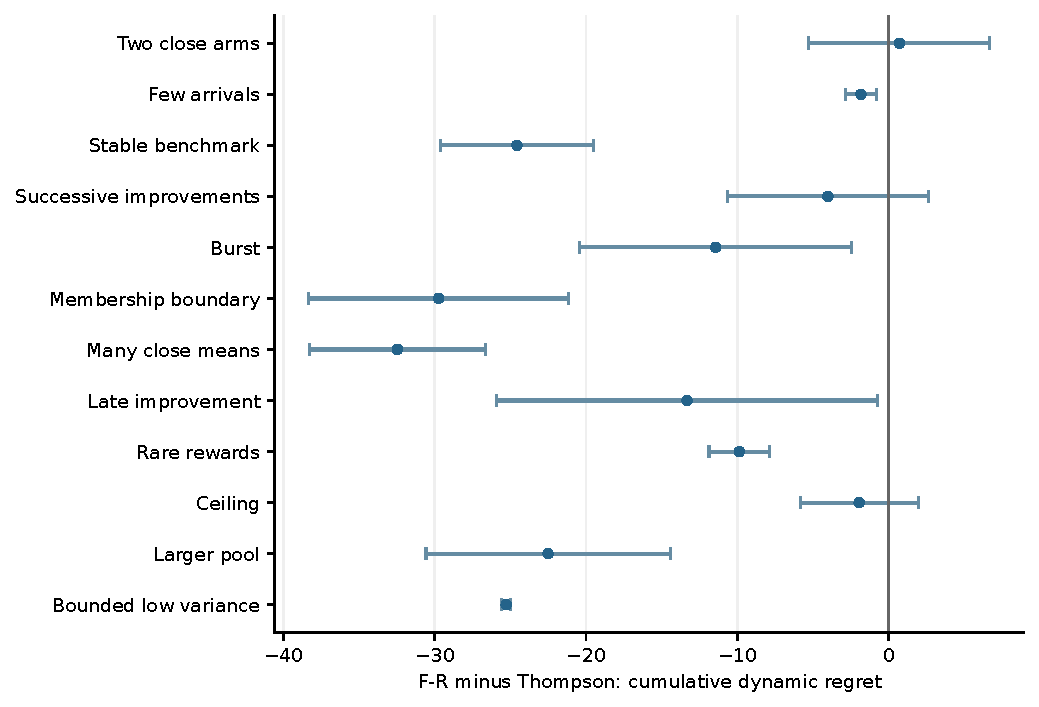
\includegraphics[width=.94\linewidth]{revision2/generated/reward-paired.pdf}
\caption{F-R minus Thompson cumulative dynamic regret in each frozen scenario. Points are means of 96 within-replication differences; error bars are individual two-sided 95\% approximate $t$ intervals. Negative differences favor F-R. These 12 intervals do not by themselves control the 60-comparison family; the adjusted counts are reported in the text.}
\label{fig:reward-paired}
\end{figure}

\subsection{Preference and certification cost}
\begin{table}[t]
\centering
\caption{Descriptive equal-weight averages of the 12 scenario means. The first six rows keep $\beta_C=1$ wherever certification is active; F-area uses no certification cap. Area is in $10^3$ arm-time units. These operating points are not an optimal frontier.}
\label{tab:preference-costs}
\small
\begin{tabular}{llrr}
\toprule
Method / preference & $\beta_C$ & Regret & Area / $10^3$ \\
\midrule
F-R & inactive & 60.73 & 62.22 \\
F, $\lambda=0.1$ & $1$ & 114.68 & 48.29 \\
F, $\lambda=0.3$ & $1$ & 213.55 & 38.46 \\
F, $\lambda=0.6$ & $1$ & 392.99 & 31.70 \\
F, $\lambda=0.9$ & $1$ & 425.03 & 30.84 \\
F, $\lambda=1$ & $1$ & 421.52 & 31.00 \\
F-area & $\infty$ & 1210.02 & 27.12 \\
CCP-original & 1 & 440.32 & 30.07 \\
ALL-auto-costmatched & 1 & 435.68 & 36.72 \\
ALL-area & $\infty$ & 1581.72 & 36.81 \\
\bottomrule
\end{tabular}
\end{table}

Increasing service preference reduces unresolved arm-time over much of the tested range, at a substantial reward cost. The points at $\lambda=.9$ and $1$ under the fixed certification budget are not monotone: the latter has slightly lower regret and slightly larger area. We retain that reversal. F-area removes the certification cap; it is a different budget configuration and is not a continuation of the same-budget curve.

Relative to ALL-auto-costmatched, F-auto-0.6 has lower equal-weight mean regret (392.99 versus 435.68) and area (31.70 versus 36.72 thousand arm-time units). The comparison with CCP-original is a trade-off: F-auto-0.6 has lower mean regret but higher mean area. F-area has lower suite mean regret and area than ALL-area. These are finite-suite averages, rather than per-scenario or pathwise Pareto guarantees. Supplementary Tables~\ref{tab:all-methods} and~\ref{tab:joint-paired} give the scenario decomposition and paired uncertainty.

\begin{figure}[t]
\centering
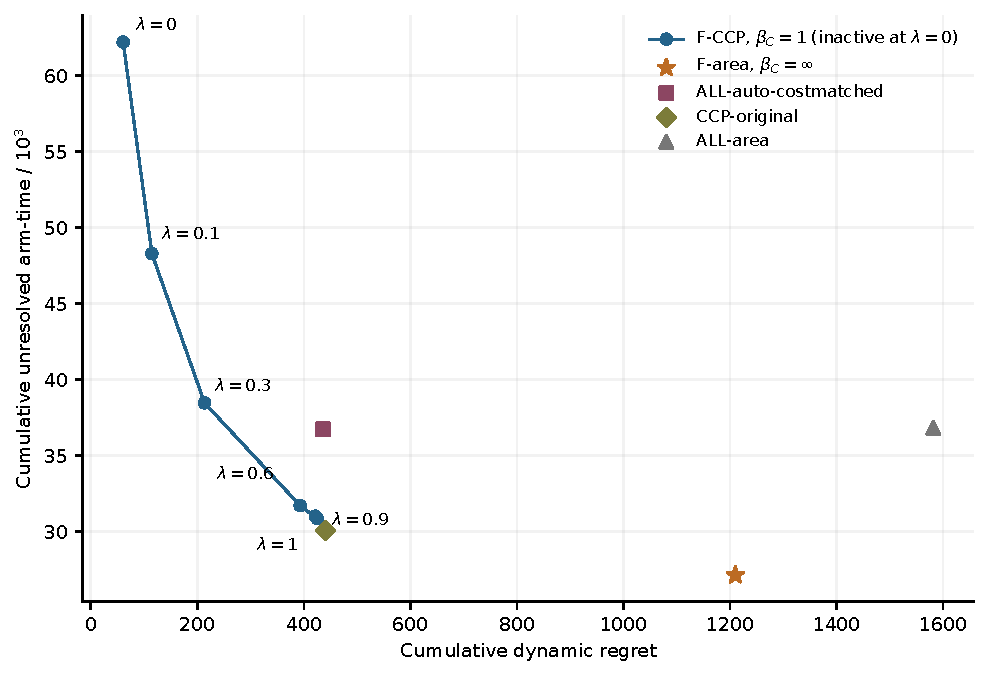
\includegraphics[width=.94\linewidth]{revision2/generated/preference-tradeoff.pdf}
\caption{Descriptive averages of terminal costs over the 12 frozen scenarios. Connected circles follow the prespecified order $\lambda=0,.1,.3,.6,.9,1$, with $\beta_R=16$, temperature $.5$, and $\beta_C=1$ whenever service is active. The star is F-area with $\beta_C=\infty$; the other markers are named comparators. The connecting segments identify configurations and do not estimate a continuous or optimal frontier. Area is divided by $10^3$.}
\label{fig:preference-tradeoff}
\end{figure}

The controller's proposed rate differs from the realized service fraction because the phase must accumulate and the certification guard can reject a proposal. Supplementary Table~\ref{tab:service-diagnostics} reports proposed busy-round rates, successful pulls, denials and the final unresolved count. Fixed-rate, uncapped-service, temperature-one and unprotected-reward variants are retained as prespecified ablations. We use those comparisons only for the mechanisms they actually change.

\subsection{Tail behavior and report failures}
\begin{table}[t]
\centering
\caption{Empirical 95th percentiles of cumulative dynamic regret from 96 replications per method and scenario. These are finite-sample tail summaries, not high-probability regret bounds.}
\label{tab:tail-and-failure}
\small
\begin{tabular}{lrr}
\toprule
Scenario & F-R & Thompson \\
\midrule
Burst & 208.887 & 123.069 \\
Ceiling & 90.940 & 48.971 \\
Larger pool & 237.301 & 184.175 \\
\bottomrule
\end{tabular}
\end{table}

The lower mean regret of F-R does not extend to all tail summaries. Its empirical 95th percentile exceeds Thompson's in the burst, ceiling and larger-pool scenarios in Table~\ref{tab:tail-and-failure}. Each percentile uses only 96 replications; it should not be read as a precise population tail estimate.

F-auto-0.6 produces an incorrect determined label on one of its 1,152 runs; F-R and F-area produce none. Coverage failures and empty intersections also occur: the respective counts are $(6,1)$ for F-R, $(7,1)$ for F-auto-0.6, and $(8,0)$ for F-area. An empty intersection triggers persistent all-unresolved reporting, not successful completion. All these runs enter the cost calculations. Since methods share potential streams, their failures are dependent and cannot be pooled as independent reliability trials. These empirical counts neither replace the reliability theorem nor justify an all-times claim from 96 repetitions. Full failure counts, empirical maxima and implementation qualifications appear in Supplementary Sections~\ref{sec:main-numerical-protocol}--\ref{sec:development-audit}.
\section{Discussion}
\label{sec:discussion}

Reliable maintenance has costs that reward allocation alone does not
measure. An uncertain arrival can obstruct many positive reports, while
a later improvement can end a fine membership task. The general lower
bounds quantify these effects. The worst-area lower bound answers a
different question and is already attained by an initial static batch;
the fixed-schedule and terminal-count growth consequences retain
different quantifiers.

F-CCP adds an implementable choice of emphasis to this task. Its evidence
layer uses every observation, its certificate planner proposes a single
next observation, and separate accounts control reward and certification
costs. Finite guards protect the spectral regret order but can reject
service; the area bound retains that rejection cost. Classification
priority with no certification guard achieves the worst-area order,
without being fastest on every instance. A compatibility endpoint
recovers a specified baseline from the start under identical state and
randomization. The default cold-temperature reward mode has a different
contract.

The frozen experiments support lower mean reward costs for F-R in most
of the specified comparisons and useful finite-budget trade-offs for
the service modes. They also show an exception in the two-arm close-mean
case, heavier empirical regret tails than Thompson sampling in three
environments, and a nonzero label-error record for the balanced mode.
Pure-reward improvements cannot be attributed to certificate scheduling
that was switched off. The corrected matched-cost ALL comparison is
distinct from the retained superseded controller result. These findings
concern the frozen suite, not uniform dominance or a general frontier.

The activation-budgeted witness characterizes an intermediate interval
on a sufficiently separated family, with an additive reward term and
its own information requirements. General causal frontiers under
unknown and overlapping arrivals remain open. The schedule-information
separation does not make every causal comparison impossible. Likewise,
the one-step zero-remainder counterexample leaves room for comparisons
with an explicit adaptation cost or a restricted performance family.

Automatic precision, reward kernels with better tail behavior, a faithful
adaptation of the original ALL-$\varepsilon$ algorithms, and large-pool
planning costs need further study. The supplement's eventual exact-set
consistency theorem belongs to a separate revisable multiresolution
procedure under finite final arrivals and strict boundary separation.
F-CCP's coverage-event completion outside a boundary band is a different
statement.

\section*{Data and code availability}
The accompanying materials contain simulated data, frozen configurations,
code, and the scripts used to generate the article's tables and figures.
The principal test has 27,648 recorded runs; a subsequent 1,152-run
matched-cost ALL correction is retained separately, together with the
superseded comparator. Replacing that comparator for the principal
analysis leaves 24 configurations and 27,648 records. Earlier checkpoint
comparisons contain 5,760 records and are reported separately in the
supplement; the preceding CCP and frontier research suites retain their
own protocols and archives. All reported failures remain in the analysis.
The available implementation distinguishes the frozen dual-account
production engine from the interactive interface and the development
branches. These materials are provided locally with the project; no
public repository or permanent archive identifier has been verified for
this version.

\bibliographystyle{plainnat}
\bibliography{references}
\end{document}
